\documentclass{report}

\usepackage[english]{babel} 
\usepackage{amsmath}
\usepackage{graphicx}

\title{IC Calibration}
\author{Arthur Adriaens}

\begin{document}
\maketitle

\section{Setup}
\begin{figure}
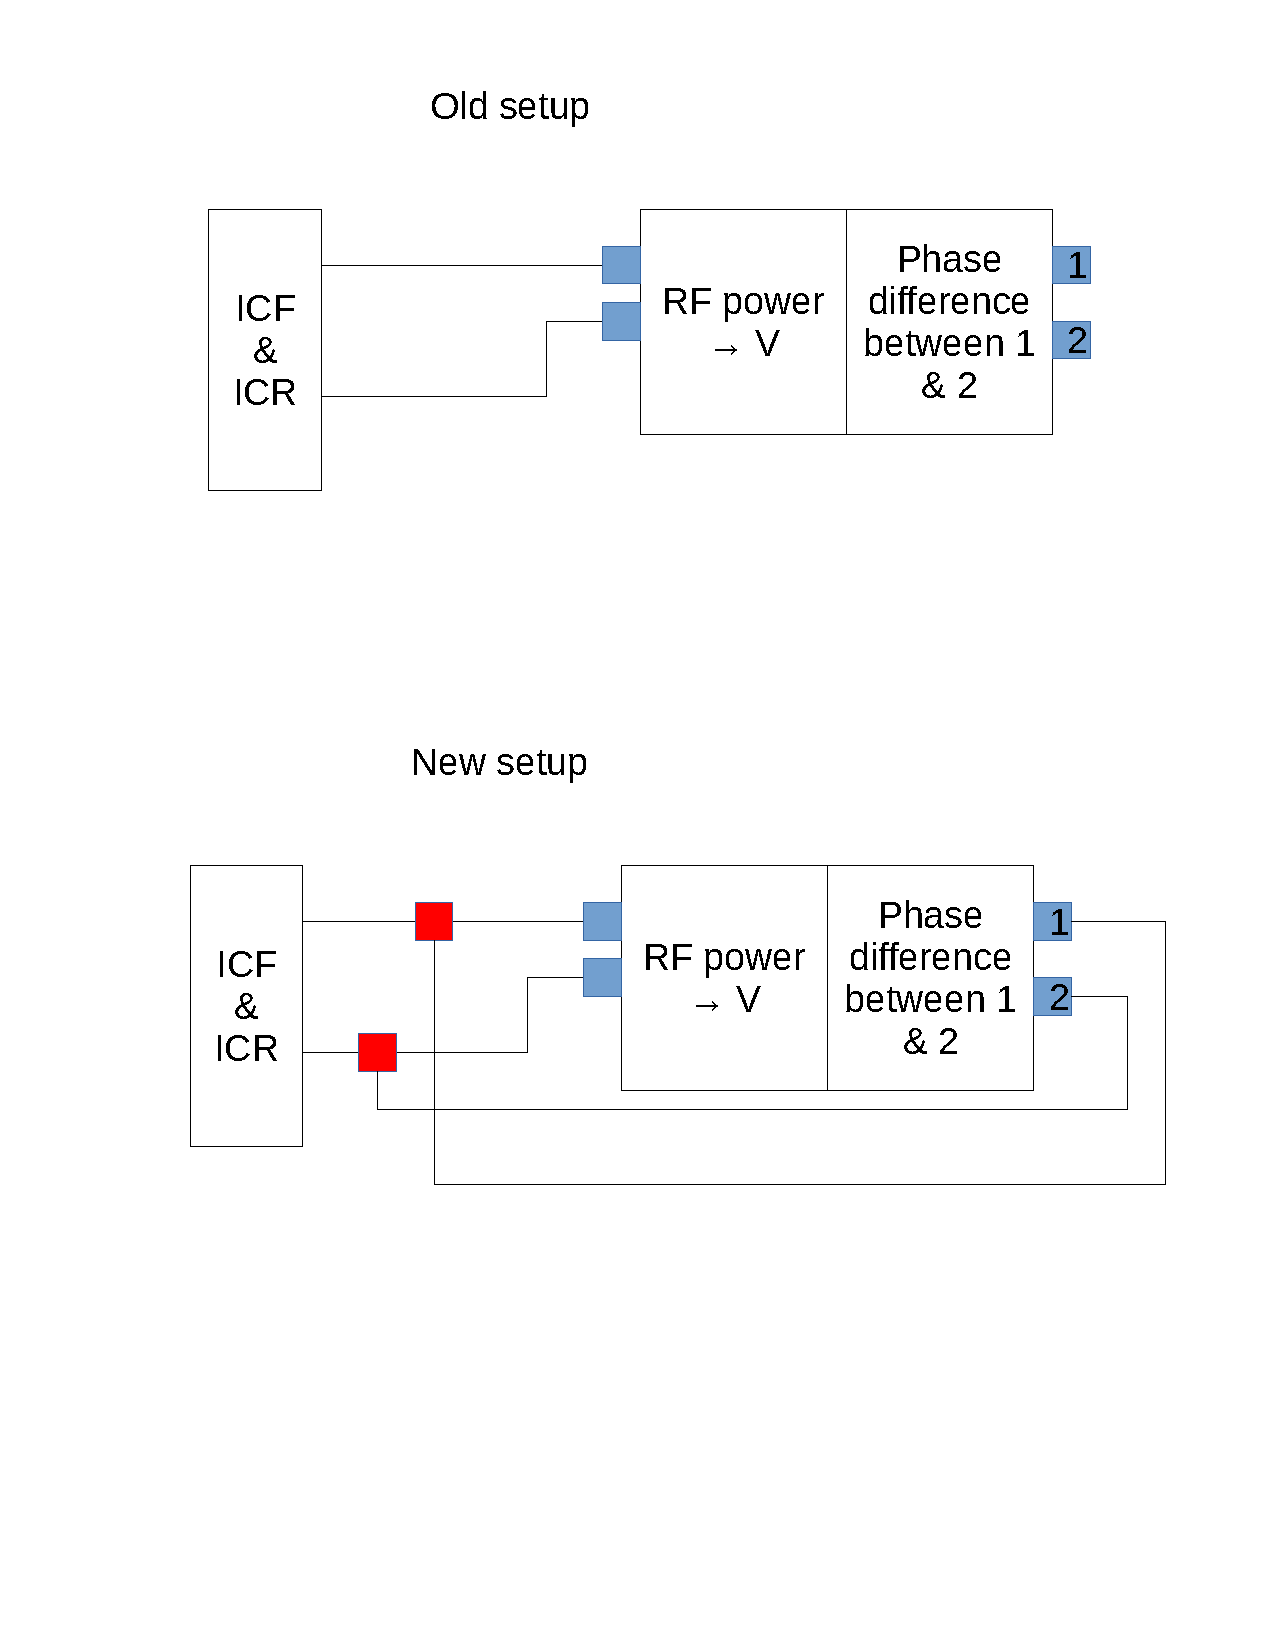
\includegraphics[width=\textwidth]{setup.pdf}
\caption{The new setup splits the signals of the forward and reflected in two, using one side to measure power and the other side to measure the phase}
\end{figure}

\section{Procedure}
\includegraphics[width=\textwidth]{figures/example_ramp.pdf}
The connectors normally connecting to the directional coupler where connected
to the VNA, after which power ramps for different frequencies were performed,
for the above shown picture this was a ramp from -20dbm to -2dbm which covers
the range of 100W to 6310W as the directional coupler induces an attenuation of
-70db (this was measured, all S-parameters and original calibration files
are available on the TOMAS github).

I then proceeded to fit a straight line to one of the ramps, this results in
a relation between time and voltage
\begin{equation}
    V = a t + b
\end{equation}
For this specific ramp we chose, the time is related to the input power as:
\begin{equation}
    P = \omega t + \rho
\end{equation}
As the ramp takes 1 second and the power difference is 18dbm, we have that 
\begin{equation}
    \omega = P_{fin} - P_{init} = 18
\end{equation}
Now using the end time of the ramp $t_{fin}$, we can find $\rho$:
\begin{equation}
    \rho = P_{fin} - (P_{fin} - P_{init}) t_{fin} = -2-18t_{fin}
\end{equation}
Now we can fill these into the relation with the voltage:
\begin{equation}
    V = \frac{a}{\omega}P - \frac{\rho a}{\omega} + b := a'P + b'
\end{equation}
I.e the relation we need is:
\begin{equation}
    P = \frac{V - b'}{a'}
\end{equation}
\section{Results}
\subsection{Old setup}
This part is useful for the people who did measurements whilst the
new box was installed prior to 13/03/24. Note that some of the
accuracy of $b$ is lost when transforming to $b'$ due to the
inaccuracy of $t_{fin}$ even though this is the case, $a'$ is still
as accurate as $a$, and as such I try to keep as many significant
digits as possible.
\begin{center}
\begin{tabular}{||c c c c c c c||}
 \hline
 Signal & a & error on a (\%) & b & error on b (\%) & $\omega$ & $t_{fin}$\\ [0.5ex]
 \hline\hline
 ICF & 0.457843 & 0.17 & 0.713159 & 0.32 & 18 & 3.348\\
 ICR & 0.442106 & 0.27 & 0.890641 & 0.36 & 18 & 3.198\\
 \hline
\end{tabular}
\end{center}
So the power we get from the voltage is:
\begin{eqnarray}
    \text{P}_{ICF}\text{(dBm)} &= \frac{V_{\text{ICF}}-2.296065}{0.02543572}\\
    \text{P}_{ICR}\text{(dBm)} &= \frac{V_{\text{ICR}}-2.1.856293}{0.02456144}
\end{eqnarray}
\subsection{New setup}
This setup is in effect as of the 13th of march 2024.
\begin{center}
    25MHz
\begin{tabular}{||c c c c c c c||}
 \hline
 Signal & a & error on a (\%) & b & error on b (\%) & $\omega$ & $t_{fin}$\\ [0.5ex]
 \hline\hline
 ICF & 0.4636 & 0.037 & 0.910352 & 0.040 & 18 & 2.673\\
 \hline
 ICR & 0.453835 & 0.083 & 0.791354& 0.126& 18 & 3.144\\
 \hline
\end{tabular}
So the power we get from the voltage is:
\begin{eqnarray}
    \text{P}_{ICF}\text{(dBm)} &= \frac{V_{\text{ICF}}-2.200913}{0.02575556}\\
    \text{P}_{ICR}\text{(dBm)} &= \frac{V_{\text{ICR}}-2.268637}{0.02521306}
\end{eqnarray}


    35MHz
\begin{tabular}{||c c c c c c c||}
 \hline
 Signal & a & error on a (\%) & b & error on b (\%) & $\omega$ & $t_{fin}$\\ [0.5ex]
 \hline\hline
 ICF & 0.464247 & 0.016 & 0.982976 & 0.031 & 18 & 2.503\\
 ICR & 0.447934& 0.09703 & 0.667036& 0.1896& 18 & 3.431\\
 \hline
\end{tabular}
\begin{eqnarray}
    \text{P}_{ICF}\text{(dBm)} &= \frac{V_{\text{ICF}}-2.196569}{0.0257915}\\
    \text{P}_{ICR}\text{(dBm)} &= \frac{V_{\text{ICR}}-2.253668}{0.02488522}\\
\end{eqnarray}

    45MHz
\begin{tabular}{||c c c c c c c||}
 \hline
 Signal & a & error on a (\%) & b & error on b (\%) & $\omega$ & $t_{fin}$\\ [0.5ex]
 \hline\hline
 ICF & 0.459813&  0.039 & 0.595329 & 0.051 & 18 & 3.353\\
 ICR & 0.446204&  0.09459& 0.935934& 0.1042& 18 & 2.822\\
 \hline
\end{tabular}
\begin{eqnarray}
    \text{P}_{ICF}\text{(dBm)} &= \frac{V_{\text{ICF}}-2.188172}{0.02554517}\\
    \text{P}_{ICR}\text{(dBm)} &= \frac{V_{\text{ICR}}-2.2447}{0.02478911}
\end{eqnarray}
\end{center}
\subsection{ICV0-3}
\begin{tabular}{||c c c c c c c||}
 \hline
 Signal & a & error on a (\%) & b & error on b (\%) & $\omega$ & $t_{fin}$\\ [0.5ex]
 \hline\hline
 ICV3 & 0.707133&  0.04609 & 0.328061 & 0.2369 & 28 & 2.764\\
 ICV2& 0.706039&  0.02707 & -0.138149 & 0.4025 & 28 & 3.4346\\
 ICV1& 0.702135&  0.02917 & 0.576769 & 0.06987 & 28 & 2.4675\\
 ICV0& 0.694397&  0.03 & 0.123464 & 0.4494 & 28 & 3.1335\\
 \hline
\end{tabular}
\end{document}
